\documentclass{article}
\usepackage{iclr2026_conference,times}
\input{math_commands.tex}

\usepackage{amssymb}
\usepackage{booktabs}
\usepackage{multirow}
\usepackage{graphicx}
\usepackage{longtable}
\usepackage{microtype}
\usepackage{xcolor}
\usepackage{xspace}
\usepackage{tikz}
\usetikzlibrary{arrows.meta,positioning}
\usepackage{hyperref}
\usepackage{url}

\title{B-FAIS: Block-Wise Forecast-Aware Imputer Selection for Time-Series Foundation Models}

\author{Anonymous Authors}

\newcommand{\bfais}{\textsc{B-FAIS}\xspace}
\newcommand{\tsfm}{TSFM}
\newcommand{\mase}{\operatorname{MASE}}
\newcommand{\native}{\textsc{native-valid}}
\newcommand{\best}{\operatorname*{arg\,min}}
\definecolor{bfblue}{RGB}{44,95,145}
\definecolor{bflight}{RGB}{232,241,248}
\hypersetup{hidelinks}
\tikzset{
  bfnode/.style={draw=bfblue, rounded corners, fill=bflight, align=center,
    minimum height=0.75cm, inner sep=3.5pt, font=\small},
  bfarr/.style={-{Latex[length=2mm]}, thick, draw=bfblue}
}

% Keep this commented for anonymous review.
% \iclrfinalcopy

\begin{document}
\maketitle

\begin{abstract}
Pretrained time-series models provide accurate forecasts without task-specific fitting, yet their numerical contexts can contain heterogeneous missing spans. Applying one imputer to an entire context assumes that the same reconstruction rule is suitable for every variable, position, and downstream forecaster. We introduce Block-wise Forecast-Aware Imputer Selection (\bfais), which represents maximal contiguous missing runs as atomic blocks and assigns an imputer to each block. A frozen time-series foundation model supplies counterfactual forecasting losses for training block-level risk rankers. At inference, a budgeted shortlist, matched pseudo-missing evidence, a sparse block-relation graph, and deterministic beam search produce a validity-gated assignment. We evaluate \bfais with TimesFM~2.5 and Chronos-2 on 30 dataset versions from 17 families, using six missingness generators, five target rates, 19 executable imputers, and 1,800 paired forecasting episodes. Family-balanced MASE is lower than ALORS, DSelect-1, NeuralUCB, and a random-valid selector; the overall difference from MetaOD is small and its confidence interval crosses zero. Against the strongest complete native single imputer selected separately for each dataset, \bfais wins on 16 of 30 versions for each forecaster. Chronos-2 nevertheless has a positive dataset-macro difference that is largely driven by large Azure errors. The evidence supports the complete forecast-aware block-wise system while showing that gains depend on the target forecaster and data family.
\end{abstract}

\section{Introduction}
\label{sec:introduction}

Time-series foundation models (TSFMs) have made inference-only forecasting practical across datasets and sampling frequencies. TimesFM uses a decoder-only patch model trained on a large time-series corpus \citep{das2024timesfm}, while Chronos maps scaled values to tokens for probabilistic forecasting \citep{ansari2024chronos}. Chronos-2 extends this line to joint multivariate and covariate-informed inputs \citep{ansari2025chronos2}. These models reduce task-specific training, yet deployment still depends on the quality of the finite context presented to the frozen forecaster. A missing interval changes local continuity, seasonal evidence, cross-variable relations, and the numerical distribution seen by the model.

Imputation is therefore part of the forecasting system rather than an isolated preprocessing choice. Classical methods impose distinct assumptions: interpolation favors local smoothness, seasonal copying favors repeated structure, chained equations exploit conditional relations, and low-rank completion exploits shared factors \citep{vanbuuren2011mice,stekhoven2012missforest,mazumder2010softimpute,yu2016trmf}. Neural imputers add recurrent, attention, generative, diffusion, and spatiotemporal inductive biases \citep{cao2018brits,fortuin2020gpvae,tashiro2021csdi,du2023saits,nie2024imputeformer}. Their reconstruction rankings need not agree with their forecasting rankings. Recent task-oriented evaluation reaches the same general conclusion and estimates downstream utility when comparing imputed series \citep{wang2024taskoriented}. A frozen TSFM creates an additional dependency: two imputations with similar reconstruction error can produce materially different forecasts because their artifacts interact differently with the pretrained model.

The appropriate imputer can also vary inside one context. A short interior gap with observations on both sides differs from a long tail outage. Synchronous gaps across correlated variables differ from isolated point loss. Selecting one algorithm for the whole episode discards this structure. Established algorithm-selection formulations map instance features to an algorithm under a performance criterion \citep{rice1976algorithm}; recent selectors learn latent task--algorithm relations, sparse expert gates, or contextual-bandit policies \citep{misir2017alors,zhao2021automatic,hazimeh2021dselect,zhou2020neuralucb}. We instantiate these mechanisms as episode-level comparators in our evaluation, while HybridLSTM uses fixed windows. Block-level decisions require explicit treatment of interactions and candidate validity.

We propose \bfais, a block-wise forecast-aware selection system for missing TSFM contexts. Each maximal contiguous missing run on one variable becomes a block. A sparse graph links adjacent, overlapping, and training-correlated blocks. Training labels come from counterfactual contexts in which a candidate replaces one block of a common anchor, and the frozen forecaster scores the resulting future. Two LambdaMART rankers estimate block--candidate risk before and after pseudo-missing evidence is available; a Huber regressor estimates pair interactions. The inference objective is solved by deterministic beam search over a shortlist of at most six candidates. Native-valid masks ensure that a numerical safety repair is never recorded as a successful candidate output.

The empirical study separates two questions. The first asks whether \bfais improves on selectors that choose or mix an imputer at sequence level. Across both forecasters, \bfais obtains a family-balanced MASE of 5.1627, compared with 6.1764 for ALORS, 6.1293 for DSelect-1, 6.3030 for NeuralUCB, and 6.1107 for random-valid selection. Its 5.1856 comparison with MetaOD yields a difference of $-0.0229$ with a confidence interval spanning zero. The second question compares \bfais with the best complete native single candidate chosen separately for each dataset. It wins on 16 of 30 dataset versions for both TimesFM~2.5 \citep{google2025timesfm25} and Chronos-2, while only TimesFM has a negative dataset-macro difference. These complementary results prevent a breadth-of-wins claim from being mistaken for universal average superiority.

The contribution is threefold. First, \bfais casts missing-context preparation as a structured assignment over contiguous blocks and models relations among them. Second, it trains the assignment with counterfactual downstream forecasting loss while using pseudo-missing reconstruction evidence at inference. Third, it evaluates block-wise selection against five complete-coverage sequence selectors, a fixed-window neural selector, and a strict per-dataset single-imputer comparator under paired rolling-origin experiments. The method and results are scoped to two frozen TSFMs and temporal extrapolation within observed dataset families.

\section{Related Work}
\label{sec:related}

\subsection{Forecasting with pretrained time-series models}

TSFMs transfer temporal representations across datasets and permit zero-shot prediction. TimesFM predicts output patches from input patches with a decoder-only architecture \citep{das2024timesfm}. Chronos treats scaled and quantized values as tokens and samples future trajectories from a pretrained sequence model \citep{ansari2024chronos}. Chronos-2 introduces group attention for information exchange across related series and directly supports multivariate contexts \citep{ansari2025chronos2}. Our study uses two operationally distinct settings: our TimesFM~2.5 adapter invokes the model independently for each target, whereas the Chronos-2 adapter passes the complete multivariate context. The distinction changes which missing blocks are visible to the forecaster and motivates model-conditioned routing.

\subsection{Time-series imputation}

Imputation methods span statistical completion and specialized temporal networks. MICE iterates conditional models \citep{vanbuuren2011mice}; MissForest uses iterative random forests \citep{stekhoven2012missforest}; SoftImpute applies nuclear-norm regularization and soft-thresholded matrix completion \citep{mazumder2010softimpute}; and TRMF augments matrix factorization with temporal regularization \citep{yu2016trmf}. Neural methods include bidirectional recurrence in BRITS \citep{cao2018brits}, a Gaussian-process latent prior in GP-VAE \citep{fortuin2020gpvae}, conditional score-based diffusion in CSDI \citep{tashiro2021csdi}, self-attention in SAITS \citep{du2023saits}, and low-rank spatiotemporal attention in ImputeFormer \citep{nie2024imputeformer}. Recent general time-series models have also been evaluated on imputation among several time-series tasks, including TimeMixer++ and TOTEM \citep{wang2025timemixerpp,talukder2024totem}; HELIX explicitly encodes variable identity and cross-dimensional synthesis \citep{zhang2026helix}. \bfais treats these methods as candidates behind a shared fit/impute interface. It does not modify their internal objectives.

Task-oriented imputation evaluates a completed sequence through the eventual analysis instead of relying only on hidden-value reconstruction. \citet{wang2024taskoriented} estimate the effect of alternative imputations on a downstream forecasting task and combine favorable values. \bfais shares the downstream-utility motivation, while its setting differs in three respects: the forecaster is frozen, the decision unit is a contiguous missing block, and training uses explicit counterfactual future loss plus a block graph. Reconstruction remains useful as an inference-time proxy because the true value and future are unavailable at deployment.

\subsection{Algorithm selection}

Algorithm selection relates instance features, a candidate set, and a performance measure \citep{rice1976algorithm}. ALORS learns latent task and algorithm factors through collaborative ranking and predicts the task representation from meta-features \citep{misir2017alors}. MetaOD uses a task--model performance matrix and maps observable task features to a latent representation \citep{zhao2021automatic}. DSelect-$k$ constructs a differentiable sparse gate over experts \citep{hazimeh2021dselect}, and NeuralUCB balances predicted reward with uncertainty in a contextual bandit \citep{zhou2020neuralucb}. HybridLSTM learns to recommend imputation procedures for local univariate windows \citep{almeida2025hybridlstm}. We adapt these ideas as controlled baselines and preserve their decision granularity: four methods and random-valid selection act on a complete episode, while HybridLSTM acts on fixed 48-step windows in our implementation. Only \bfais detects data-dependent missing blocks and assigns different registered candidates within one episode.

\section{Problem Setup}
\label{sec:problem}

Let $X\in\mathbb{R}^{T\times D}$ be a complete multivariate trajectory and $M\in\{0,1\}^{T\times D}$ an observation mask. The corrupted trajectory is $\widetilde X=M\odot X+(1-M)\odot\mathrm{NaN}$. For forecast origin $t$, context length $L$, horizon $H$, and target set $\mathcal K$, an episode contains
\begin{equation}
 C_t=\widetilde X[t-L:t],\qquad
 Y_t=X[t:t+H,\mathcal K].
\end{equation}
A frozen forecaster $f$ maps a completed context $Z\in\mathbb{R}^{L\times D}$ to $\widehat Y=f(Z)$. The candidate set $\mathcal A$ contains fitted or stateless imputers. Candidate $a$ produces a completed tensor $Z^a$ and a native-valid mask that states where the candidate itself returned finite values before any safety repair.

For each variable, every maximal contiguous run of zeros in the context mask is an atomic block $b=(d,s_b,e_b)$ with length $\ell_b=e_b-s_b$. The block set is $\mathcal B$. A block-wise assignment $\mathbf a=(a_b)_{b\in\mathcal B}$ forms $Z(\mathbf a)$ by copying candidate $a_b$ on block $b$ and restoring all observed entries from $C_t$. The desired deployment policy minimizes the expected forecasting loss of $f(Z(\mathbf a))$ subject to candidate availability and a finite inference budget. The training procedure observes clean futures at earlier origins; deployment and final evaluation do not expose future values to the router.

We use target-macro MASE \citep{hyndman2006another}. For target $k$, the scale $s_k$ is computed only from the training prefix using the registered seasonal lag $q_k$, with lag one used when the prefix is too short:
\begin{equation}
s_k=\max\!\left(\epsilon,\frac{1}{T_{\rm tr}-q_k}
\sum_{u=q_k+1}^{T_{\rm tr}}|X_{u,k}-X_{u-q_k,k}|\right),
\end{equation}
\begin{equation}
\mathcal L_f(Z,Y)=\frac{1}{|\mathcal K|}\sum_{k\in\mathcal K}
\frac{H^{-1}\sum_{h=1}^{H}|Y_{h,k}-f(Z)_{h,k}|}{s_k}.
\end{equation}

\section{B-FAIS}
\label{sec:method}

Figure~\ref{fig:overview} summarizes training and inference. Training constructs forecast-aware unary and pair labels from clean historical episodes. Inference first estimates prior risks, runs a small candidate shortlist, measures pseudo-missing behavior, and solves a structured assignment. A final model-specific calibration was frozen on the ETT development family and is reported separately from the learned router.

\begin{figure}[t]
\centering
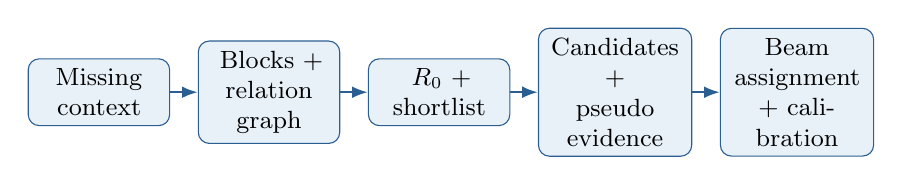
\begin{tikzpicture}[node distance=3.5mm]
\node[bfnode, text width=1.55cm] (ctx) {Missing\\context};
\node[bfnode, text width=1.55cm, right=of ctx] (graph) {Blocks +\\relation graph};
\node[bfnode, text width=1.55cm, right=of graph] (r0) {$R_0$ +\\shortlist};
\node[bfnode, text width=1.7cm, right=of r0] (r1) {Candidates +\\pseudo evidence};
\node[bfnode, text width=1.7cm, right=of r1] (solve) {Beam assignment\\+ calibration};
\draw[bfarr] (ctx) -- (graph);
\draw[bfarr] (graph) -- (r0);
\draw[bfarr] (r0) -- (r1);
\draw[bfarr] (r1) -- (solve);
\end{tikzpicture}
\caption{\bfais inference. Training replaces the unavailable final future with earlier clean futures and labels block--candidate counterfactuals through the frozen forecaster.}
\label{fig:overview}
\end{figure}

\subsection{Sparse block relation graph}

The graph $G=(\mathcal B,\mathcal E)$ encodes interactions that a collection of independent block decisions would miss. It contains three edge types. Same-variable neighboring blocks receive weight $1/(1+\mathrm{gap})$. Blocks on different variables are linked when they overlap or touch in time, with overlap normalized by the larger block length. A third edge connects temporally nearby blocks whose variables have high absolute correlation in the training prefix, and its weight decays with temporal gap. Cross-variable degree limits keep synchronous point loss from producing a dense graph. If an episode contains more than 512 blocks, inference omits pair terms and reports the fallback in its artifact.

\subsection{Counterfactual forecast teacher}

LOCF supplies a common complete anchor $A$. For block $b$ and candidate $a$, $A^{b\leftarrow a}$ replaces only $b$ with candidate values. The local counterfactual effect is
\begin{equation}
\delta^{\rm local}_{b,a}=\mathcal L_f(A^{b\leftarrow a},Y)-\mathcal L_f(A,Y).
\end{equation}
Local substitutions can understate a candidate's global behavior. Let $Z^a$ be the context completed entirely by $a$, let $\bar\delta^{\rm global}_a=(\mathcal L_f(Z^a,Y)-\mathcal L_f(A,Y))/|\mathcal B_{\rm vis}|$, and let $\mathcal B_a$ be blocks where $a$ is natively valid. The calibrated unary label is
\begin{equation}
\widetilde R_{b,a}=\delta^{\rm local}_{b,a}+\bar\delta^{\rm global}_a
-\frac{1}{|\mathcal B_a|}\sum_{b'\in\mathcal B_a}\delta^{\rm local}_{b',a}.
\label{eq:teacher}
\end{equation}
When a candidate covers every visible block, summing Equation~\ref{eq:teacher} recovers its complete-context loss increment. Interactions use a second-order counterfactual difference,
\begin{align}
\Phi_{bc}(a,a')={}&\mathcal L_f(A^{b\leftarrow a,c\leftarrow a'},Y)
-\mathcal L_f(A^{b\leftarrow a},Y)\nonumber\\
&-\mathcal L_f(A^{c\leftarrow a'},Y)+\mathcal L_f(A,Y).
\end{align}
The teacher samples at most four blocks, six candidates, and four pair labels per training episode. These caps limit TSFM calls and mean that training never exhaustively labels every assignment.

\subsection{Two-stage risk estimation and shortlist}

The prior ranker $R_0(b,a)$ uses block geometry, boundary availability, local and global missing rates, variable correlations, candidate capabilities and measured costs, data-family and mechanism identifiers, and forecaster descriptors. Both $R_0$ and the refined ranker $R_1$ are LightGBM LambdaMART models \citep{burges2010lambdamart,ke2017lightgbm}, with candidates for one block forming a ranking group. A LightGBM Huber regressor estimates $\Phi_{bc}$ from edge, block-pair, candidate-pair, coverage, and output-summary features.

Inference constructs a shortlist $S$ of at most six candidates before expensive evidence refinement. LOCF and linear interpolation are always retained. Each remaining candidate is greedily scored by the reduction in the best predicted $R_0$ risk across blocks divided by one plus its measured cost. This is the operational compute control in the reported experiments. Although the generic assignment objective contains an activation-cost term, its final coefficient is zero.

The selected candidates run on the actual context and on eight pseudo-missing blocks drawn from the observed training history. Pseudo blocks preferentially match the real block's variable, length, and relative position; cross-variable pseudo masks avoid temporal overlap. Their native reconstruction MAE, RMSE, bias, coverage, and uncertainty augment the feature vector for $R_1$. The final unary score normalizes evidence within each block and combines $R_0$, $R_1$, pseudo-missing error, and a training-time candidate prior. The forecaster-specific weights are frozen before confirmatory evaluation and listed in Appendix~\ref{app:method-details}.

\subsection{Structured assignment and validity-gated assembly}

For shortlisted, natively valid candidates, \bfais minimizes
\begin{equation}
E(\mathbf a)=\sum_{b\in\mathcal B}R(b,a_b)
+\beta\!\sum_{(b,c)\in\mathcal E}w_{bc}\widehat\Phi_{bc}(a_b,a_c)
+\gamma\!\sum_{a\in\mathcal A}\mathbb I[a\text{ used}]c_a.
\label{eq:energy}
\end{equation}
We use deterministic beam search with width 32, $\beta=1$, and $\gamma=0$. Exhaustive search appears only in small correctness tests. A candidate may be assigned to a block only if every missing position in that block is natively valid. If no shortlisted candidate satisfies this constraint, a separate repair state applies linear interpolation, LOCF, or the training median. Repair values maintain a finite tensor and are never counted as native candidate success. Assembly restores the original observed values before the TSFM receives the context.

\subsection{Frozen TSFM-specific calibration}
\label{sec:calibration}

The final system includes inference rules selected on the four ETT versions. TimesFM~2.5 chooses a forecast medoid per target among LOCF, linear interpolation, seasonal lag, and Kalman AR completions. When the pseudo-missing best candidate exceeds the structured completion by a relative risk margin of 0.05, the two contexts are blended with weight 0.5; natively valid seasonal-lag values then receive a 0.1 shrinkage weight. Chronos-2 averages the two candidates with greatest forecast consensus, shrinks natively valid blocks toward seasonal lag with weight 0.9, and uses linear interpolation with weight 0.75 only when seasonal lag is unavailable. These rules are part of the evaluated system. They are distinguished from the learned block router because the repository does not contain a confirmatory component-removal study.

\section{Experimental Setup}
\label{sec:experiments}

\paragraph{Data and missingness.}
The data audit accepted 32 dataset versions and retained 30 versions from 17 families; Housing Inventory was too short and Job Claims had no valid evaluation origin after the temporal split. The collection combines ETT benchmarks \citep{zhou2021informer} with series represented in the Monash archive \citep{godahewa2021monash} and additional public energy, labor, transport, cloud, coastal, and supply-chain series. Context length, forecast horizon, and rolling stride are all 96, and the first two variables are forecasting targets. A corruption mask is generated once on the complete sequence for each dataset, item, mechanism, rate, and seed, then sliced at every origin. Consequently, an origin does not receive a favorable redraw. Six synthetic stress tests cover random points, independent blocks, synchronous blocks, staggered correlated blocks, value-dependent loss, and mixed outages at target missing rates $\{0.1,0.2,0.3,0.4,0.5\}$. These labels describe generators rather than asserting a data-generating mechanism in the sense of \citet{rubin1976inference}. The balanced evaluation manifest contains 30 episodes per dataset and forecaster, or 900 per forecaster and 1,800 paired episodes overall.

The four ETT versions serve as development data for the forecaster-specific calibration in Section~\ref{sec:calibration}; the other 26 versions are confirmatory for those rules. Within every version, supervised router labels use earlier origins and evaluation uses later origins, following rolling-origin practice \citep{tashman2000outofsample}. This design measures temporal extrapolation within observed dataset families. It does not measure transfer to an unseen family.

\paragraph{Candidates and comparators.}
The executable pool contains 19 imputers: simple temporal rules, Kalman and Gaussian-process models, multivariate statistical completion, and recent neural imputers. TRMF is registered but disabled because the available transductive interface does not match the rolling protocol. Candidate-specific native-valid masks are retained throughout evaluation. We compare with ALORS, MetaOD, DSelect-1, NeuralUCB, and an episode-level random-valid selector. Each comparator is adapted to the common candidate outputs and episode features; Appendix~\ref{app:baselines} records deviations from its source formulation. HybridLSTM is analyzed separately because its fixed ten-imputer pool and failed outputs leave only 1,322 of 1,800 episodes valid.

\paragraph{Forecasters, metrics, and inference.}
We freeze TimesFM~2.5 and Chronos-2 without task-specific parameter updates. The local checkpoint mapping uses \path{google/timesfm-2.5-200m-pytorch} \citep{google2025timesfm25} and \path{amazon/chronos-2} \citep{ansari2025chronos2}. Our TimesFM adapter invokes the model independently for each target; Chronos-2 receives the multivariate context and returns predictive quantiles, from which we use the median as the point forecast. The primary statistic is target-macro MASE, then an equal-weight mean over the 17 dataset families. We pair methods on identical episodes. Confidence intervals use 2,000 hierarchical bootstrap resamples over family, dataset version, and item--mask unit. Family-level paired Wilcoxon tests are adjusted within each reported view over six registered selector comparisons, including the separately reported HybridLSTM analysis, by Holm's procedure \citep{holm1979simple}. The primary view uses all 1,800 windows: 1,706 contain at least one missing context value, while 94 are zero-block no-op episodes produced by slicing the full-sequence mask. The missing-window-only view in Appendix~\ref{app:stratified-results} preserves the main interpretation. The strict single-imputer comparison additionally requires one candidate to be natively complete for the entire episode and chooses the best such candidate separately for each dataset. Router and search settings are fixed at a six-candidate shortlist, eight pseudo blocks, beam width 32, $\beta=1$, and $\gamma=0$; further implementation details are in Appendix~\ref{app:method-details}.

\section{Results}
\label{sec:results}

\subsection{Comparison with sequence-level selectors}

Table~\ref{tab:selector-main} reports the primary family-balanced comparison. The sign convention is $\Delta=\mase_{\text{\bfais}}-\mase_{\text{comparator}}$, so negative values favor \bfais. Its overall MASE is 5.1627. The confidence intervals exclude zero against ALORS, DSelect-1, NeuralUCB, and random-valid selection, and the corresponding family-level tests remain below 0.05 after Holm adjustment. The difference from MetaOD is $-0.0229$ with an interval spanning zero. Thus the evidence distinguishes \bfais from four comparators while supporting only similar aggregate performance to MetaOD.

\begin{table}[t]
\centering
\small
\setlength{\tabcolsep}{4.2pt}
\caption{Family-balanced selector comparison across both forecasters. \bfais MASE is 5.1627; all methods have 1,800 paired episodes. Negative $\Delta$ favors \bfais.}
\label{tab:selector-main}
\begin{tabular}{lrrrrr}
\toprule
Comparator & MASE & $\Delta$ & 95\% CI & Family win & $p_{\rm Holm}$ \\
\midrule
ALORS & 6.1764 & $-1.0136$ & $[-2.3757,-0.2332]$ & .941 & .0004 \\
DSelect-1 & 6.1293 & $-0.9665$ & $[-2.4830,-0.1483]$ & .941 & .0006 \\
MetaOD & 5.1856 & $-0.0229$ & $[-0.2217,+0.2132]$ & .647 & .4307 \\
NeuralUCB & 6.3030 & $-1.1403$ & $[-2.9257,-0.1810]$ & .765 & .0063 \\
Random-valid & 6.1107 & $-0.9480$ & $[-2.0657,-0.2528]$ & .941 & .0004 \\
\bottomrule
\end{tabular}
\end{table}

The direction is similar when the forecasters are separated, with important uncertainty differences. For TimesFM, \bfais has MASE 2.4205 and intervals excluding zero against all comparators except MetaOD. For Chronos-2, it has MASE 7.9050; intervals exclude zero against ALORS and NeuralUCB, while DSelect-1, MetaOD, and random-valid cross zero. Appendix~\ref{app:stratified-results} gives the complete estimates. By missing rate, the margins over most selectors become larger at rates 0.4 and 0.5, whereas MetaOD remains close at every rate. Across mechanisms, no single generator explains the aggregate ranking.

HybridLSTM returns a valid result on 73.4\% of episodes. Among its 1,322 valid episodes, the error distribution is extremely heavy-tailed, primarily because of the fifth-order spline candidate. Reporting its conditional mean in Table~\ref{tab:selector-main} would change the evaluation population, so Appendix~\ref{app:coverage} treats this outcome as a coverage and stability result. Mean end-to-end episode time is 3.5669 seconds for \bfais and 3.5249--3.7351 seconds for the complete-coverage comparators on the recorded workstation. These times are descriptive because the artifact does not record the GPU model.

\subsection{Comparison with complete single imputers}

The strict comparison asks a different question: for each dataset, can \bfais beat the post hoc best candidate that produced a natively complete context on every evaluated episode? This comparator has access to per-dataset outcome rankings and is stronger than deploying one globally fixed imputer. Table~\ref{tab:strict-main} shows 16 wins in 30 versions for each forecaster and 12 wins among the 26 non-ETT versions. TimesFM has a negative macro difference, while Chronos-2 has a positive macro difference despite the same win count. The Chronos result is driven by a small number of high-error versions, particularly an Azure series with $\Delta=+33.5039$. The strict evidence therefore supports broad competitiveness and exposes a material tail-risk limitation; it does not establish uniform average improvement.

\begin{table}[t]
\centering
\small
\setlength{\tabcolsep}{5pt}
\caption{Strict comparison with the best complete native single imputer selected separately for each dataset. Negative macro $\Delta$ favors \bfais.}
\label{tab:strict-main}
\begin{tabular}{lrrrr}
\toprule
Forecaster & Wins & Non-ETT & Macro $\Delta$ & Non-ETT $\Delta$ \\
\midrule
TimesFM 2.5 & 16/30 & 12/26 & $-0.1255$ & $-0.1339$ \\
Chronos-2 & 16/30 & 12/26 & $+1.4521$ & $+1.6875$ \\
\bottomrule
\end{tabular}
\end{table}

These two evaluations answer complementary questions. The selector comparison evaluates the complete \bfais system against episode-level adaptations on the same population; it does not isolate the effect of decision granularity. The strict comparator tests whether the structured system can exceed the strongest complete candidate on each dataset. The first comparison is favorable except for a statistical tie with MetaOD; the second reveals nearly balanced wins and forecaster-dependent macro behavior. Appendix~\ref{app:strict-results} reports every dataset-level difference so that the long-tailed failures remain visible.

\section{Limitations}
\label{sec:limitations}

The study evaluates two frozen TSFMs and trains router labels on earlier origins from the same dataset versions later used for evaluation. The four ETT versions also determine forecaster-specific consensus and shrinkage rules. Results consequently establish temporal extrapolation under fixed dataset families, missingness generators, and checkpoints. Transfer to new families, new TSFMs, or naturally occurring missingness remains untested.

The final system combines the learned block router with hand-selected TSFM-specific calibration. The repository contains development variants, yet it does not contain a confirmatory component-removal study for the relation graph, pair regressor, pseudo blocks, shortlist, consensus rule, or shrinkage. Those variants cannot support causal attribution among components. The positive Chronos strict macro difference further indicates that model-specific safeguards require improvement. The activation-cost coefficient is zero in the reported configuration, so computational restraint comes from shortlisting rather than an optimized accuracy--cost tradeoff.

Deep candidates use the common training budget available in this repository, including ten epochs for several neural imputers. Different budgets could change candidate rankings. Learned selectors were not refit under multiple training seeds, the strict comparison lacks a paired confidence interval, and the timing artifact omits the GPU model. HybridLSTM uses its own fixed pool and has incomplete coverage, which prevents an equal-population accuracy comparison. Finally, raw datasets, external model checkpoints, and large result artifacts are not all tracked in the source tree; exact replication requires those assets and their licenses.

\section{Conclusion}
\label{sec:conclusion}

\bfais assigns imputers to contiguous missing blocks using counterfactual forecasting supervision, pseudo-missing evidence, a sparse relation graph, and validity-gated structured search. Across 1,800 paired episodes, it improves family-balanced MASE over four complete-coverage sequence selectors and is statistically indistinguishable from MetaOD. It also wins against the best complete native single candidate on 16 of 30 dataset versions for each of two TSFMs, although Chronos-2 has unfavorable macro behavior because of large failures on a few datasets. These results establish the feasibility and competitiveness of the complete block-wise forecast-aware system while identifying calibration, tail risk, unseen-family transfer, and formal component analysis as the principal next tests.

\bibliographystyle{iclr2026_conference}
\bibliography{tsfm_fais_iclr2026}

\appendix
\section{Detailed Experimental Protocol}
\label{app:protocol}

This appendix records the protocol represented by the frozen configuration files and formal result artifacts. It separates registered options from settings that were actually executed. Development variants in the artifact tree are not treated as confirmatory experiments.

\subsection{Rolling-origin construction}

Table~\ref{tab:protocol} summarizes the common episode construction. Complete source sequences are first split temporally. A deterministic full-sequence mask is generated for each dataset, item, mechanism, rate, and seed before rolling windows are cut. The same realization is therefore reused across eligible origins and all evaluated methods. Imputers and routers receive only the corrupted context and training-prefix summaries. The clean future is available to the counterfactual teacher at earlier training origins and to the evaluator at held-out origins; it is unavailable during final imputation and routing.

\begin{table}[h]
\centering
\small
\caption{Common rolling-origin protocol. Caps are maxima because short series and candidate validity can reduce the realized count.}
\label{tab:protocol}
\begin{tabular}{ll}
\toprule
Setting & Value \\
\midrule
Context / horizon / forecast stride & 96 / 96 / 96 \\
Training-window stride & 24 \\
Training prefix & first 20\% of each sequence \\
Target variables & registered indices 0 and 1 \\
Items per dataset & at most 4 \\
Train / evaluation origins per item & at most 4 / 4 \\
Teacher episodes per dataset & at most 30 \\
Evaluation episodes per dataset and TSFM & 30 \\
Mechanisms / target rates & 6 / $\{.1,.2,.3,.4,.5\}$ \\
Final mask seeds & 22, 33, 44 \\
Global configuration seed & 20260710 \\
Dataset versions / families & 30 / 17 \\
TSFMs / total paired episodes & 2 / 1,800 \\
\bottomrule
\end{tabular}
\end{table}

Of the 1,800 primary-view windows, 1,706 contain at least one missing value in the 96-step context. The remaining 94 windows are legitimate zero-block episodes arising when a full-sequence mask has no missing cell inside a particular context slice. Every selector performs a no-op on those episodes. We retain them in the prespecified all-windows view and report a missing-window-only sensitivity view in Appendix~\ref{app:stratified-results}.

\subsection{Synthetic missingness generators}

The target missing count is computed over the complete $T\times D$ array. Table~\ref{tab:mechanisms} gives the implemented construction. Block lengths are drawn from the registered length set. If a block placement cannot reach the exact target count, remaining cells are sampled uniformly from still-observed positions. These are controlled stress tests and are not claims about the natural missingness process of any source dataset.

\begin{table}[h]
\centering
\small
\caption{Implemented synthetic missingness generators.}
\label{tab:mechanisms}
\begin{tabular}{p{0.25\linewidth}p{0.66\linewidth}}
\toprule
Generator & Construction \\
\midrule
Random point & Uniform sampling without replacement over observed cells. \\
Independent block & Random channel, start, and block length for each placement. \\
Synchronous block & Shared missing time spans across all variables, followed by exact-count repair if needed. \\
Staggered correlated & Select highly correlated variables from the calibration prefix and shift related blocks around a common start. \\
Value dependent & Rank cells by robust absolute deviation from a calibration median and place blocks around high-score cells. \\
Mixed outage & Allocate about 70\% of the target count to independent blocks and the remainder to random points. \\
\bottomrule
\end{tabular}
\end{table}

\subsection{Dataset inventory and audit exclusions}

The data audit accepted 32 versions. \path{Housing_Inventory_M} was excluded because its length is 114, which cannot support the registered split, context, and horizon. \path{Job_Claims_W} contains 196 points but has no eligible evaluation origin after the prefix/origin constraints. Table~\ref{tab:data-inventory} lists the 30 evaluated versions. The four ETT versions form the development family for the TSFM-specific calibration; all other versions are confirmatory for those rules. Earlier origins from every listed version are still used for supervised router construction, so this is not an unseen-family split.

\begin{table}[h]
\centering
\small
\caption{Evaluated dataset families and versions.}
\label{tab:data-inventory}
\begin{tabular}{p{0.27\linewidth}p{0.64\linewidth}}
\toprule
Family & Dataset versions \\
\midrule
Azure 2019 & \path{azure2019_D_5T}, \path{azure2019_I_5T}, \path{azure2019_U_5T} \\
Coastal TS & \path{Coastal_T_S_15T}, \path{Coastal_T_S_20T}, \path{Coastal_T_S_H} \\
Current velocity & \path{current_velocity_5T}, \path{current_velocity_15T}, \path{current_velocity_20T}, \path{current_velocity_H} \\
Electricity & \path{electricity} \\
ETT (development) & \path{ETTh1}, \path{ETTh2}, \path{ETTm1}, \path{ETTm2} \\
EWELD load & \path{EWELD_Load_15T} \\
Exchange rate & \path{exchange_rate} \\
JOLTS & \path{JOLTS_M} \\
National illness & \path{national_illness} \\
NE China wind & \path{NE_China_Wind_H} \\
OpenElectricity NEM & \path{OpenElectricity_NEM_5T} \\
Port activity & \path{Port_Activity_D}, \path{Port_Activity_W} \\
Supply chain & \path{Supply_Chain_Customer_D}, \path{Supply_Chain_Location_D} \\
Traffic & \path{traffic} \\
Uncertainty & \path{Uncertainty_1M_M} \\
US labor & \path{US_Labor_M} \\
Vehicle & \path{Vehicle_Sales_M}, \path{Vehicle_Supply_M} \\
\bottomrule
\end{tabular}
\end{table}

\subsection{Candidate pool and native validity}
\label{app:candidates}

The registry contains 20 entries. TRMF is disabled because the installed PyPOTS~1.5 wrapper exposes a transductive interface that is inconsistent with the rolling fit/impute contract. The remaining 19 candidates are executed. Table~\ref{tab:candidates} groups them by operational family; this grouping is descriptive and does not merge their outputs.

\begin{table}[h]
\centering
\small
\caption{Executed imputation candidates.}
\label{tab:candidates}
\begin{tabular}{p{0.25\linewidth}p{0.66\linewidth}}
\toprule
Group & Candidates \\
\midrule
Temporal rules & LOCF, linear interpolation, seasonal lag \\
State-space and GP & Kalman local trend, Kalman AR, STL--Kalman, GP--RBF \\
Multivariate statistical & KNN, MICE, MissForest, SoftImpute \\
Specialized neural & BRITS, GP-VAE, SAITS, CSDI, ImputeFormer, HELIX \\
General time-series & TimeMixer++, TOTEM \\
\bottomrule
\end{tabular}
\end{table}

Candidate completion is evaluated before the common numerical repair. GP-VAE, ImputeFormer, KNN, SAITS, SoftImpute, TimeMixer++, and TOTEM are natively valid in all 1,800 selector episodes. CSDI, HELIX, and MICE are valid in 1,740; MissForest in 1,680; LOCF and the Kalman family in approximately 1,636; seasonal lag in only 246. These differences arise from requirements such as available boundary values, sufficient seasonal history, finite model output, and dimensional caps. A repaired value can keep the TSFM input finite, but it never changes a candidate's native-valid status or comparison coverage.

\section{Method and Implementation Details}
\label{app:method-details}

\subsection{Feature groups}

The router uses registered numeric and categorical descriptors rather than raw future values. Table~\ref{tab:feature-groups} records the feature groups used by the prior ranker, refined ranker, and pair regressor. Candidate output summaries are computed only on the available context or on pseudo-hidden observed values.

\begin{table}[h]
\centering
\small
\caption{Feature groups used by the routing models.}
\label{tab:feature-groups}
\begin{tabular}{p{0.24\linewidth}p{0.67\linewidth}}
\toprule
Group & Examples \\
\midrule
Block geometry & variable, start/end, length, relative position, boundary availability, local missing rate \\
Episode context & global missing rate, variable count, seasonal period, training-prefix summaries, family and mechanism identifiers \\
Candidate descriptors & family, mode, fit scope, tail/period capability, stochastic flag, device and measured cost \\
Pseudo evidence & native coverage, MAE, RMSE, bias, uncertainty, and matched pseudo-block geometry \\
Pair descriptors & edge type/weight, overlap or gap, correlation, block-pair geometry, candidate pair, coverage, and output summaries \\
Forecaster descriptors & registered TSFM identity, target granularity, context mode, and output type \\
\bottomrule
\end{tabular}
\end{table}

The counterfactual teacher labels at most four blocks and six candidates per training episode, plus at most four pair labels. This sampling cap makes the teacher computationally finite and also limits supervision for rare block--candidate combinations. Candidate priors require at least four supporting examples.

\subsection{Frozen routing and search settings}

\begin{table}[h]
\centering
\small
\caption{Frozen B-FAIS settings used for both confirmatory runs.}
\label{tab:bfais-settings}
\begin{tabular}{ll}
\toprule
Component & Setting \\
\midrule
Prior / refined unary model & LightGBM LambdaMART / LambdaMART \\
Pair model & LightGBM Huber regression \\
Shortlist size / forced candidates & 6 / LOCF and linear interpolation \\
Pseudo blocks & 8 \\
Beam width & 32 \\
Pair coefficient $\beta$ & 1.0 \\
Activation-cost coefficient $\gamma$ & 0.0 \\
Candidate-switch penalty & 0.0 \\
Pair fallback & omit pair terms above 512 blocks \\
Internal repair order & linear interpolation, LOCF, training median \\
Tail repair order & LOCF, training median \\
\bottomrule
\end{tabular}
\end{table}

The evaluated activation-cost coefficient is zero. Compute restraint is supplied by the six-candidate shortlist and teacher sampling caps. The cost-aware greedy shortlist score remains active because it divides marginal prior-risk coverage by one plus measured candidate cost. The energy itself does not impose an additional cost penalty.

The final evidence blend is forecaster specific. For TimesFM~2.5, the normalized weights on $(R_0,R_1,\text{pseudo proxy},\text{global prior})$ are $(0.1,0.1,0.3,0.5)$. For Chronos-2 they are $(0.0,0.1,0.2,0.7)$. The four ETT versions are the registered tuning family for these values.

\subsection{Frozen forecast calibration}

The TimesFM adapter invokes the local 2.5 checkpoint independently for each target. Target-wise calibration considers LOCF, linear interpolation, seasonal lag, and Kalman AR completions. It selects the forecast medoid, optionally blends the structured and pseudo-best contexts with weight 0.5 when the relative pseudo-risk margin is at least 0.05, and shrinks natively valid seasonal-lag cells with weight 0.1.

The Chronos-2 adapter passes up to eight target-and-correlate variables as one multivariate context. It obtains predictive quantiles and uses the median quantile for point MASE. Calibration averages the two candidate contexts with greatest forecast-value consensus, shrinks natively valid cells toward seasonal lag with weight 0.9, and uses linear interpolation with weight 0.75 when seasonal lag is unavailable. These rules are part of the reported systems; no confirmatory removal experiment isolates their contribution.

\section{Baseline Adaptations}
\label{app:baselines}

The selector baselines are adaptations to a common offline imputer-selection setting. Their original papers motivate the selection mechanisms; the exact training schedule, episode features, validity handling, and candidate outputs below belong to this repository. The first four methods and random-valid selection act on a complete episode. HybridLSTM acts on fixed univariate windows and retains its own candidate set.

\begin{table}[h]
\centering
\small
\caption{Baseline implementations used in the selector comparison.}
\label{tab:baseline-adaptations}
\begin{tabular}{p{0.19\linewidth}p{0.72\linewidth}}
\toprule
Method & Repository adaptation \\
\midrule
MetaOD & Eight-dimensional latent task representation, ten optimization epochs, and a 100-tree random forest from episode features to latent coordinates. The implementation omits per-epoch forest refitting and validation early stopping. \\
ALORS & Ten-dimensional collaborative factors, ten epochs, NDCG cutoff 10, and a ten-tree random forest for new-task factors. Alternating Adam replaces the source optimizer. \\
DSelect-1 & One selected expert ($k=1$), 100 epochs, and differentiable binary-code gating. Probability assigned to an unavailable expert is redistributed across candidates that are natively valid for the episode. \\
NeuralUCB & Hidden width 100, ridge coefficient 1, exploration coefficient 1, and one update per round. The implementation retains the full precision matrix through Woodbury updates. \\
Random-valid & Uniform episode-level sampling from candidates that are natively valid for the entire episode. The configuration identifier contains ``block,'' while the realized method is sequence level. \\
HybridLSTM & Univariate windows of length 48, ten internal imputers, and 800 training epochs. It does not use the common 19-candidate pool. The source study also considers longer windows, so 48 is an implementation setting. \\
\bottomrule
\end{tabular}
\end{table}

The common selector training target is imputation loss for the adapted baselines, whereas B-FAIS learns from counterfactual forecast loss and adds its frozen calibration. Differences in Table~\ref{tab:selector-main} therefore compare complete systems. They cannot identify the isolated effect of block granularity, target construction, or calibration.

\section{Additional Selector Results}
\label{app:stratified-results}

\subsection{Forecaster strata}

Table~\ref{tab:forecaster-strata} reports the same family-balanced statistic separately for each frozen forecaster. Chronos-2 has larger MASE levels and wider intervals. The sign convention remains B-FAIS minus comparator.

\begin{table}[h]
\centering
\small
\caption{Family-balanced selector results by forecaster. B-FAIS MASE is 7.9050 for Chronos-2 and 2.4205 for TimesFM~2.5.}
\label{tab:forecaster-strata}
\begin{tabular}{llrrr}
\toprule
Forecaster & Comparator & Comparator MASE & $\Delta$ & 95\% CI \\
\midrule
Chronos-2 & ALORS & 9.0120 & $-1.1070$ & $[-2.5621,-0.1833]$ \\
 & DSelect-1 & 8.8078 & $-0.9028$ & $[-2.4529,+0.1245]$ \\
 & MetaOD & 7.9547 & $-0.0497$ & $[-0.2242,+0.0991]$ \\
 & NeuralUCB & 9.2382 & $-1.3332$ & $[-4.2818,-0.1233]$ \\
 & Random-valid & 8.6873 & $-0.7823$ & $[-1.8105,+0.0160]$ \\
\midrule
TimesFM 2.5 & ALORS & 3.3408 & $-0.9203$ & $[-2.2837,-0.1619]$ \\
 & DSelect-1 & 3.4507 & $-1.0302$ & $[-2.5534,-0.1327]$ \\
 & MetaOD & 2.4166 & $+0.0039$ & $[-0.2836,+0.3969]$ \\
 & NeuralUCB & 3.3679 & $-0.9474$ & $[-2.4594,-0.1193]$ \\
 & Random-valid & 3.5341 & $-1.1136$ & $[-2.5064,-0.2822]$ \\
\bottomrule
\end{tabular}
\end{table}

\subsection{Windows containing missing values}

Removing the 94 zero-block episodes leaves 1,706 paired windows for each complete-coverage comparator. Table~\ref{tab:missing-window-view} shows that the interpretation is unchanged: four intervals exclude zero and MetaOD remains close to B-FAIS.

\begin{table}[h]
\centering
\small
\caption{Family-balanced sensitivity analysis on windows with at least one missing context value. B-FAIS MASE is 5.2553.}
\label{tab:missing-window-view}
\begin{tabular}{lrrr}
\toprule
Comparator & Comparator MASE & $\Delta$ & 95\% CI \\
\midrule
ALORS & 6.2919 & $-1.0366$ & $[-2.3444,-0.2630]$ \\
DSelect-1 & 6.2518 & $-0.9965$ & $[-2.6390,-0.1522]$ \\
MetaOD & 5.2758 & $-0.0205$ & $[-0.2319,+0.2037]$ \\
NeuralUCB & 6.4399 & $-1.1846$ & $[-2.9741,-0.1758]$ \\
Random-valid & 6.2410 & $-0.9857$ & $[-2.0919,-0.2449]$ \\
\bottomrule
\end{tabular}
\end{table}

\subsection{Missingness mechanisms}

Table~\ref{tab:mechanism-results} reports the all-windows family macro by generator. The first numeric column is the B-FAIS MASE; subsequent columns are B-FAIS minus comparator. MetaOD remains close under all six generators. Differences against the other selectors vary in magnitude, which argues against attributing the aggregate result to one mechanism.

\begin{table}[h]
\centering
\scriptsize
\setlength{\tabcolsep}{3.8pt}
\caption{Results by missingness generator. Negative differences favor B-FAIS.}
\label{tab:mechanism-results}
\begin{tabular}{lrrrrrr}
\toprule
Generator & B-FAIS & MetaOD & DSelect & NeuralUCB & ALORS & Random \\
\midrule
Independent block & 4.9544 & $+.0199$ & $-.8290$ & $-1.2817$ & $-.8456$ & $-.5294$ \\
Mixed outage & 4.7834 & $+.1360$ & $-.5589$ & $-1.9970$ & $-1.0222$ & $-.2770$ \\
Random point & 4.2943 & $+.0137$ & $-1.1497$ & $-.6818$ & $-.8691$ & $-.3540$ \\
Staggered correlated & 5.0730 & $-.1305$ & $-1.4625$ & $-.6988$ & $-1.5692$ & $-1.6984$ \\
Synchronous block & 5.5820 & $-.2281$ & $-1.3587$ & $-.4312$ & $-.2197$ & $-.5233$ \\
Value dependent & 6.2893 & $+.0515$ & $-.4404$ & $-1.7515$ & $-1.5561$ & $-2.3057$ \\
\bottomrule
\end{tabular}
\end{table}

\subsection{Target missing rates}

Table~\ref{tab:rate-results} gives the corresponding rate strata. The differences from DSelect-1, NeuralUCB, ALORS, and random-valid selection generally become larger at rates 0.4 and 0.5. MetaOD remains within 0.25 MASE of B-FAIS in every rate stratum. No monotonic claim is made about the absolute B-FAIS MASE because dataset composition and mask realization remain part of each family macro.

\begin{table}[h]
\centering
\scriptsize
\setlength{\tabcolsep}{4.2pt}
\caption{Results by target missing rate. Negative differences favor B-FAIS.}
\label{tab:rate-results}
\begin{tabular}{rrrrrrr}
\toprule
Rate & B-FAIS & MetaOD & DSelect & NeuralUCB & ALORS & Random \\
\midrule
.1 & 4.6712 & $+.2497$ & $+.1203$ & $+.2543$ & $-.2741$ & $-.0212$ \\
.2 & 5.1959 & $-.0268$ & $-.9002$ & $-1.6937$ & $-.0568$ & $+.0782$ \\
.3 & 4.7317 & $-.0903$ & $-.6682$ & $-.4760$ & $-1.6066$ & $-.4415$ \\
.4 & 5.3874 & $-.1249$ & $-.8167$ & $-.8065$ & $-.7406$ & $-1.4484$ \\
.5 & 5.8274 & $-.1222$ & $-2.5679$ & $-2.9797$ & $-2.3902$ & $-2.9071$ \\
\bottomrule
\end{tabular}
\end{table}

\section{Coverage, Stability, and Runtime}
\label{app:coverage}

Table~\ref{tab:runtime-coverage} separates result coverage from recorded end-to-end episode time. All methods in the main selector table cover the same 1,800 episodes. HybridLSTM covers 1,322, and its mean time is conditional on a different internal pool and the successful subset. It is therefore unsuitable for either an equal-population accuracy claim or a direct speed ranking.

\begin{table}[h]
\centering
\small
\caption{Selector coverage and descriptive episode runtime.}
\label{tab:runtime-coverage}
\begin{tabular}{lrrr}
\toprule
Method & Valid / 1,800 & Coverage & Mean time (s) \\
\midrule
B-FAIS & 1,800 & 100.0\% & 3.5669 \\
ALORS & 1,800 & 100.0\% & 3.5275 \\
DSelect-1 & 1,800 & 100.0\% & 3.5249 \\
MetaOD & 1,800 & 100.0\% & 3.5397 \\
NeuralUCB & 1,800 & 100.0\% & 3.7351 \\
Random-valid & 1,800 & 100.0\% & 3.5249 \\
HybridLSTM & 1,322 & 73.4\% & 0.1952 \\
\bottomrule
\end{tabular}
\end{table}

On HybridLSTM's valid subset, family-balanced MASE is 4.8500 for B-FAIS and 4,767.9798 for HybridLSTM. The large conditional mean is primarily associated with the fifth-order spline option, and 239 episodes per forecaster have no valid HybridLSTM output. We report these facts as an implementation stability result rather than a general conclusion about the source method.

The strict imputation stages record totals of 2,776.73 seconds for the TimesFM run and 2,766.14 seconds for the Chronos run. The environment artifact records Windows~10, Python~3.10.20, and PyTorch~2.5.1+cu124, but no GPU model. Hardware-normalized throughput, energy consumption, and candidate-level TSFM-call counts cannot be recovered from the retained artifacts.

\section{Dataset-Level Strict Comparison}
\label{app:strict-results}

For each dataset and forecaster, the strict comparator is the candidate with the lowest evaluation MASE among candidates that are natively complete for every episode of that dataset. The table lists that candidate and $\Delta=\mase_{\text{B-FAIS}}-\mase_{\text{best single}}$. This is a post hoc per-dataset comparator, not one fixed imputer chosen before deployment.

\footnotesize
\begin{longtable}{p{0.31\linewidth}p{0.15\linewidth}rp{0.15\linewidth}r}
\caption{Per-dataset strict comparison. Negative differences favor B-FAIS.}
\label{tab:strict-dataset}\\
\toprule
Dataset & TimesFM best & $\Delta$ & Chronos best & $\Delta$ \\
\midrule
\endfirsthead
\multicolumn{5}{c}{\tablename\ \thetable\ (continued)}\\
\toprule
Dataset & TimesFM best & $\Delta$ & Chronos best & $\Delta$ \\
\midrule
\endhead
\midrule
\multicolumn{5}{r}{Continued on next page}\\
\endfoot
\bottomrule
\endlastfoot
Coastal\_T\_S\_15T & helix & $-0.2830$ & timemixerpp & $-0.0719$ \\
Coastal\_T\_S\_20T & helix & $-4.1009$ & mice & $+2.8480$ \\
Coastal\_T\_S\_H & helix & $-0.1019$ & helix & $-0.0835$ \\
ETTh1 & saits & $-0.0742$ & saits & $-0.0969$ \\
ETTh2 & helix & $-0.0706$ & helix & $-0.0619$ \\
ETTm1 & gpvae & $-0.0133$ & mice & $-0.0743$ \\
ETTm2 & helix & $-0.1234$ & helix & $-0.0798$ \\
EWELD\_Load\_15T & mice & $-0.0115$ & saits & $-0.0010$ \\
JOLTS\_M & mice & $+0.1940$ & mice & $+0.6825$ \\
NE\_China\_Wind\_H & softimpute & $+0.1865$ & softimpute & $+0.2226$ \\
OpenElectricity\_NEM\_5T & saits & $+0.2123$ & knn\_multivariate & $-0.0445$ \\
Port\_Activity\_D & saits & $-0.1248$ & saits & $-0.1237$ \\
Port\_Activity\_W & locf & $-0.0009$ & kalman\_ar & $+0.0366$ \\
Supply\_Chain\_Customer\_D & mice & $+0.4365$ & mice & $+0.2879$ \\
Supply\_Chain\_Location\_D & mice & $+0.0564$ & mice & $-0.0200$ \\
US\_Labor\_M & mice & $-1.5705$ & mice & $-0.6373$ \\
Uncertainty\_1M\_M & knn\_multivariate & $+0.1590$ & timemixerpp & $+0.2175$ \\
Vehicle\_Sales\_M & missforest & $-0.1216$ & mice & $-0.2353$ \\
Vehicle\_Supply\_M & csdi & $+0.1825$ & mice & $-0.3591$ \\
azure2019\_D\_5T & saits & $+0.0520$ & softimpute & $+7.0614$ \\
azure2019\_I\_5T & kalman\_ar & $-0.0096$ & saits & $+0.4306$ \\
azure2019\_U\_5T & saits & $-0.0605$ & softimpute & $+33.5039$ \\
current\_velocity\_15T & helix & $+0.0094$ & helix & $+0.0551$ \\
current\_velocity\_20T & missforest & $+0.0007$ & missforest & $+0.0955$ \\
current\_velocity\_5T & saits & $+0.0348$ & saits & $-0.0473$ \\
current\_velocity\_H & knn\_multivariate & $-0.0053$ & softimpute & $+0.0973$ \\
electricity & imputeformer & $-0.0035$ & imputeformer & $-0.0310$ \\
exchange\_rate & helix & $+1.1520$ & helix & $-0.2057$ \\
national\_illness & mice & $+0.0571$ & mice & $+0.0409$ \\
traffic & mice & $+0.1780$ & missforest & $+0.1560$ \\
\end{longtable}
\normalsize

The TimesFM differences have mean $-0.1255$ and maximum $+1.1520$ on \path{exchange_rate}. The Chronos differences have mean $+1.4521$ and maximum $+33.5039$ on \path{azure2019_U_5T}. Excluding all three Azure versions reduces the Chronos mean to approximately $+0.0951$, so Azure errors dominate the magnitude without fully determining its sign. The available strict artifacts do not contain a paired confidence interval or multiplicity-adjusted test.

\section{Evidence Boundaries and Reproducibility}
\label{app:reproducibility}

\subsection{Experiments that are absent}

The repository contains many router and calibration variants used for development and schema regression. It does not contain a confirmatory one-at-a-time removal study for the block relation graph, pair term, pseudo blocks, shortlist, evidence blend, forecast consensus, shrinkage, or target granularity. It also lacks multiple independent training seeds for learned selectors, a sensitivity analysis for the ten-epoch neural-imputer budget, an unseen-family split, results for more than two real TSFM checkpoints, and a hardware-complete cost analysis. No numerical component claim in this paper is derived from development variants.

\subsection{Artifacts and replication scope}

The source tree provides configuration files, dataset manifests, routing and evaluation code, and tests. The primary selector statistics come from \path{family_macro_comparison_summary.csv} in the formal comparison directory below. Strict results come from the final TimesFM and Chronos evaluation directories named in the repository documentation.
\begin{center}
\small\path{artifacts/main-selector-sequence-comparison-v2/}
\end{center}
The artifact directory, raw datasets, external checkpoints, and large generated tensors are excluded from version control in a fresh checkout. Exact numerical replication therefore requires the local assets used by the recorded runs, plus verification of their source terms and checksums.

The frozen forecaster mappings are recorded as follows:
\begin{center}
\small TimesFM: \path{google/timesfm-2.5-200m-pytorch}\qquad
Chronos-2: \path{amazon/chronos-2}
\end{center}
Evaluation never downloads a replacement checkpoint silently. The point prediction for Chronos-2 is the returned median quantile. All observed context cells are restored after block assembly, and native validity is evaluated before fallback repair. These checks should be retained in any reproduction because relaxing them changes both eligibility and coverage.

\subsection{Data and responsible use}

The study uses archival or publicly distributed time-series collections and does not involve an intervention, human-subject recruitment, or intentional processing of personal information. Synthetic masks are added to complete numerical arrays. Dataset ownership and licensing remain with the original providers; authors should verify redistribution terms before publishing raw files. Forecasting errors can carry operational consequences in energy, labor, logistics, and infrastructure settings, and the reported research system should not be used as an autonomous decision rule without domain-specific validation and monitoring.

\subsection{Generative AI disclosure}

Generative AI tools assisted with literature-metadata checking, language editing, LaTeX drafting, and consistency review. The authors remain responsible for the experimental claims, source verification, interpretation, and final manuscript. No generated numerical result is presented as experimental evidence; every reported value is transcribed from a repository artifact and was checked against its formal summary.

% CAMERA-READY TODO: replace Anonymous Authors with the verified author list,
% affiliations, and corresponding-author details.
% CAMERA-READY TODO: add verified CRediT roles, funding statement,
% acknowledgments, and conflict-of-interest statement after author approval.


\end{document}
